\chapter{Related Works}

\section{Data Mining}

Data mining \cite{zaki2010advances, han2011data} is an interdisciplinary subfield of computer science and statistics, which can discover patterns and inferences in large datasets. These patterns contain valuable information about the data, from which different conclusions can be drawn for the dataset. Data mining is a tool for information extraction, processing, representation and summarization. 

\medskip \noindent There are five stages that can be mentioned in connection with data processing:
\begin{verse}
	$\bullet$ Selection: Features with the highest perceived information value need to be selected.\\
	$\bullet$ Preprocessing: The dataset may include errors, missing values or inconsistent data that need to be filtered out.\\
	$\bullet$ Transformation: Some features of the dataset require transformation, such as normalization, in order to be processable by data mining or machine learning models.\\
	$\bullet$ Data mining: Data mining techniques need to be used that can discover the patterns.\\
	$\bullet$ Evaluation: The patterns are known, therefore it can be seen, that not all of the patterns are needed for the prediction.
\end{verse}

Data mining has applications in multiple fields, which not only encompasses scientific research but industrial applications such as banking, business, insurance, production engineering and so on. It can help companies to develop more effective strategies in a more optimal way.



\subsection{The Dataset}

Selecting the information that can be useful for the dataset needs a thorough examination. A well-defined dataset is large in scale and carries a lot of information whereof patterns can be predicted. Collecting enough relevant data is a long process, but there are public datasets that can be used for free. \medskip

Online News Popularity dataset \cite{Fernandes2015API, onlinenews-url} - which is a prediction of Mashable news popularity - is publicly available at UCI Machine Learning repository. It provides the popularity of online news, and neural networks can predict the future popularity of the news articles from given information before the release of news articles. 

\begin{figure}[h]
	\centering
	\caption{The Online News Popularity dataset of Mashable news is served by UCI Machine Learning Repository.}
	
\includegraphics[height=0.15\linewidth]{./figures/mashable}
	\label{fig:mashable}
\end{figure}

The UCI Machine Learning Repository \cite{uci-url} is a collection of datasets as a service to the machine learning community. These datasets can be used for free to various machine learning tasks.\smallskip

Mashable is a digital media website that was founded in 2005. Online News Popularity dataset \cite{Ren2015PredictingAE} contains information about 40.000 articles published between 2013 and 2015 on Mashable's website. \smallskip

Online News Popularity dataset consists of 58 predictive features, 2 other attributes of accessory information and 1 goal field, which is the number of shares. The dataset was preprocessed before its publication, where general transformation steps were made. The dataset originally contained nominal features like the day of the publication or the type of the data channel, but they were transformed by one-hot encoding prior to publication. After the encoding, the predictive features are numeric values. Three types of keywords such as worst, average and best were captured by ranking all articles keyword average shares. Additionally, a bunch of natural language processing features were extracted such as closeness to top Latent Dirichlet Allocation (LDA) topics, title subjectivity, the rate of positive and negative words and title sentiment polarity. Sentiment polarity and subjectivity scores were also computed.\smallskip

Online News Popularity dataset meets all the requirements for a regression problem and its preprocessing and transformation has already made before its publication. However the dataset is not prepared for applying data mining techniques, it needs more cleaning.



\section{Machine Learning}

Machine learning \cite{mitchell1997machine, michalski2014machine, alpaydin2009introduction} is a field of artificial intelligence that gives computers the capability to learn from past data to help predict current or future states of a system. Learning relies on patterns and inferences, instead of explicit instructions. Machine learning utilizes statistical methods to process predefined datasets and to predict future output values for given data inputs. \medskip

Fields of application and popularity have been substantial in the recent years. Machine learning can be used during data processing, from the feature selection phase, to the application of data mining methods, as machine learning models are built from data mining techniques.  \medskip

There are well-known techniques that can be used after analysing and optimizing the data. Two of the most widely adopted machine learning methods are supervised learning and unsupervised learning.

\subsubsection{Supervised Learning}

\label{para:supervised}Supervised learning provides labeled training data, which are used during the prediction phase. Supervised learning's algorithm analyses the given dataset and processes the labeled data for mapping new examples. There are several types of supervised learning that can be divided into two main classes that are classification and regression. In \textbf{classification}, the samples can only be discrete types, but in \textbf{regression}, the desired output consists of one or more continuous variables and real numbers.

\subsubsection{Unsupervised Learning}

Unsupervised learning is another category of the learning problem, in which the training data consists of a set of input vectors without any corresponding target values. One of the goals in these problems may be to discover groups of similar attributes within the dataset, which is called \textbf{clustering}.



\subsection{Biological Nervous Systems}

The neural network \cite{feldman2013neural} is a system with the functionalities of the human brain. It can recognize patterns and process real-world data with respect of these patterns.\smallskip

Learning processes in artificial neural networks originate from the behavior of human brain and nervous system. In a biological brain, neurons communicate with electrical signals. Each neuron has several branches, called dendrites, which generate these signals that are sent through axons to other neurons. Neurons can communicate by their synapses, when the passed signal fires. Firing mechanism of the neuron contains two states. Namely, an off state in which the neuron does not transmit signals, and an on state of the signal, which helps the signal to pass from a neuron's synapses to another. With this sustained operation, signals are processed through a number of other neurons before reaching their destination.
\begin{figure}[h]
	\centering
	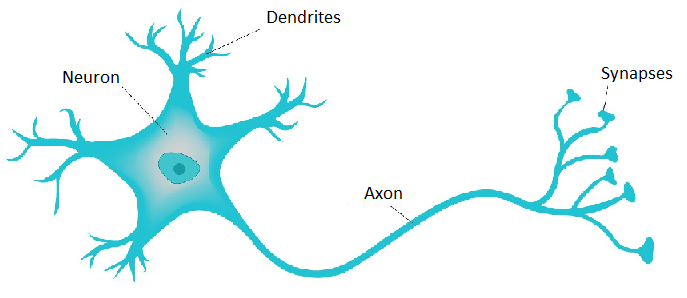
\includegraphics[height=0.35\linewidth]{./figures/neuron2}
	\caption{The biological neuron's structure}
	\label{fig:neuron}
\end{figure}



\subsection{Artificial Neural Networks}

The artificial neural network \cite{priddy2005artificial, anastassiou2011intelligent} is a model of machine learning. For a simple explanation, it is a machine learning tool, which utilizes different learning functions to gather knowledge and solve various machine learning problems. An artificial neural network uses artificial neurons to model the complex process of the human brain. During the learning process, these neurons receive inputs, then change their internal state, which is called activation, to produce the desired outputs. This activation phase - similarly to the synapses - processes the given inputs from one neuron to another. \medskip

The artificial neural network itself is not an algorithm, but rather a framework for many different machine learning algorithms that can process complex data inputs. These learning algorithms learn from the experiences that are obtained from processing many examples. Each process yields an output, which, depending on the other outputs can determine which characteristics of the input are needed to construct the correct output. If there are a sufficient number of processed examples, the neural network can generate potential inputs and see if they produce the correct outputs. As the quantity of training data increases, so does the learning time and complexity of the neural network, however, training data also potentially increases the estimation accuracy. \medskip

A general classification task for artificial neural networks is the problem of image recognition. For example, it can be trained to identify whether or not the picture contains a rabbit. The system was manually programmed with showing example images, which was labeled as it contains a rabbit, or not. This process helps the system to identify rabbits on other pictures. The system can accomplish this without any task-specific rules, like any knowledge about how a rabbit looks like. Instead they automatically generate identifying characteristics from the patterns that they processed.\medskip

The fields of artificial neural networks' application are quite wide. As already mentioned, image/pattern recognition, but also self driving vehicle trajectory prediction, data mining, email spam filtering, signature verifications, medical diagnosis, cancer research, deep neural networks and several other areas use it nowadays. Some of those examples include Amazon which uses neural networks to power their recommendation engines, Microsoft for their translation services, Facebook for facial recognition and Google across many of its products including Google Translate and Gmail (spam filters). Essentially neural networks can be applied to a broad range of problems and can process many different types of input, including images, videos, files and databases among many others. 



\subsection{Neural Network Inversion}

There is a subfield of machine learning that has not received much attention since the rise of deep learning. This subfield is the neural network inversion problem \cite{KINDERMANN1990277}. 

\label{para:inversion}Neural network inversion procedures seek to find one or more input values that produce a desired output response for a fixed set of synaptic weights. Although the inversion of a neural network propounds various problems, because in case of a given dataset several inputs can produce the same output. This means, that when an artificial neural network is made to learn a dataset, it will rarely be invertible. Since the artificial neural networks behave as a universal function approximator, they can learn any function with the infinite number of artificial neurons. Thus neural network inversion consists of the procedures which can approximate one or more points from the input set with respect of the examined output. \medskip

There are several methods which can perform neural network inversion which can be placed into three broad classes. Exhaustive search should be considered, when the dimensionality of the input and allowable range of each input variable is low. Single element inversion methods are used to find one inversion point per process. Multi element inversion procedures are able to find numerous inversion points simultaneously. \medskip

Inversion of the neural network can be useful in many areas which uses machine learning. For example, a single element inversion task is the problem of sonar performance under various environmental conditions \cite{article}. A neural network is trained to generate SIR pixel values as a function of sonar and environmental parameters. Once trained, the inverted neural network can provide input parameters to generate desired SIR performance in a specified target region.



\section{Python}

\begin{figure}[h]
	\centering
	\caption{Python and its library Scikit-Learn with the assistance of Anaconda are appropriate platforms to train artificial neural networks}
	
\includegraphics[height=0.25\linewidth]{./figures/python_scikit}
	\label{fig:python_scikit}
\end{figure}

Python \cite{vanderplas2016python, python-url} is an interpreted, object-oriented, high-level programming language with dynamic semantics, used for general-purpose programming. It was created by Guido van Rossum and released in 1991. \medskip

\noindent Several goals have been defined for Python \cite{van2011introduction}:
\begin{verse}
	$\bullet$ an easy and intuitive language;\\
	$\bullet$ open source, so anyone can contribute to its development;\\
	$\bullet$ code that is easily readable;\\
	$\bullet$ suitable for everyday tasks, allowing for short development times.
\end{verse}
Due to the realization of these goals, Python is said to be one of the most popular programming languages nowadays. It is easy to learn, has efficient high-level data structures and a simple but effective approach to object-oriented programming. Python's elegant syntax and dynamic typing, together with its interpreted nature, make it an ideal language for scripting and rapid application development in many areas on most platforms.\medskip

\textbf{Anaconda} is the interpreter of Python, which contains more than 1500 built-in packages for Python. Anaconda provides a distribution for scientific computing, for example executing data mining or machine learning tasks. Anaconda has a package manager system called conda, that helps to facilitate the various scientific tasks.\medskip

In the artificial intelligence community, Python is one of the most used language, due to its effectivity. Numerous artificial intelligence fields' researchers develop in Python, with the assistance of the built-in libraries and several other sources found on the internet. The usefulness of Python for data science comes primarily from the large and active third-party packages:  
\begin{verse}
	- \textbf{SciPy} for containing a wide array of numerical tools such as numerical integration and interpolation;
	
	- \textbf{Scikit-Learn} for providing a uniform toolkit for applying common machine learning algorithms to data;
	
	- \textbf{NumPy} for providing efficient storage and computing multi-dimensional data arrays;
	
	-  \textbf{Pandas} for providing a DataFrame object along with a powerful set of methods to manipulate, filter, group, and transform data; 
	
	- \textbf{Matplotlib} for providing a useful interface for creating publication-quality plots and figures;
\end{verse} 
and many more tools that aimed scientific computing and other machine learning fields. Also the vast majority of the libraries used for data science have Python interfaces.\\ 
Besides the prebuilt libraries, choosing Python for artificial intelligence programming can make the development easier and faster with the specific indenting style and the dynamic typing system, which means less coding and more developing. Python is platform independent, its interpreter and extensive standard library are available in source or binary form for free.

At last one of the core benefits of Python is its flexibility. With options to choose from either scripting and OOP approach, Python is suitable for every purpose. Moreover, it also works as a perfect backend language and linking different data structures together is also suitable in Python.